\documentclass{article}

\usepackage{microtype}
\usepackage{graphicx}
\usepackage{booktabs}
\usepackage{hyperref}

% Not anonymized (the course does not require double-blind review).
\usepackage[preprint]{icml2026}

\usepackage{amsmath}
\usepackage{amssymb}
\usepackage{amsthm}
\usepackage{enumitem}
\usepackage{xcolor}
\usepackage[capitalize,noabbrev]{cleveref}

\newcommand{\todo}[1]{\textcolor{red}{[TODO: #1]}}

\icmltitlerunning{Self-Consistency as an Unsupervised Post-Training Signal for VQA}

\begin{document}

\twocolumn[
  \icmltitle{Self-Consistency as an Unsupervised Post-Training Signal\\for Visual Question Answering}

  \begin{icmlauthorlist}
    \icmlauthor{Matthew Bernard}{ucb}
    \icmlauthor{Shiqi Yang}{ucb}
  \end{icmlauthorlist}

  \icmlaffiliation{ucb}{University of California, Berkeley, CA, USA}

  \icmlcorrespondingauthor{Matthew Bernard}{mattb@berkeley.edu}
  \icmlcorrespondingauthor{Shiqi Yang}{shiqiy@berkeley.edu}

  \icmlkeywords{Unsupervised post-training, self-consistency, pseudo-labeling, vision-language models, VQA}

  \vskip 0.3in
]

\printAffiliationsAndNotice{}

\begin{abstract}
Unsupervised post-training adapts a pre-trained model without human labels by letting the model generate its own training signal. We study whether self-consistency can serve as such a signal for a small vision-language model on visual question answering. Using SmolVLM-500M-Instruct on the image-based questions of ScienceQA, we read the model's probability over the answer options in a single forward pass, keep training questions whose confidence exceeds a threshold, and fine-tune the model on its own predictions with LoRA. Along the way, we find that the position at which option probabilities are read matters: an instruction-tuned model places only 7\% of its probability on the option letters at the end of the prompt, and prefilling ``Answer:'' fixes this. Confidence filtering raises pseudo-label accuracy on the validation split from 64.2\% to 74.3\% at $\tau = 0.9$. Fine-tuning on these pseudo-labels, however, leaves test accuracy unchanged (64.8\%, versus 65.8\% without filtering; neither differs significantly from the base model) and makes the model more confident on its wrong answers. Fine-tuning on ground-truth labels for the same questions reaches 77.2\%. Self-consistency therefore mostly reinforces what the model already believes, which is the mechanism behind error propagation in self-training.
\end{abstract}

\section{Introduction}

Post-training has become the standard way to adapt pre-trained foundation models to downstream tasks. Instead of the massive corpora used in pre-training, post-training relies on smaller, targeted data, for example through supervised instruction tuning \citep{wei2022flan}, preference-based alignment \citep{ouyang2022instructgpt}, or reinforcement learning \citep{chu2025sft}. Most of these methods still depend on human-provided labels or preferences, which are costly to collect and unavailable for many new tasks and domains. This motivates \emph{unsupervised} post-training, in which the model generates its own training signal from unlabeled inputs.

A natural source of such a signal is \emph{self-consistency}: when a model is sampled several times on the same input, agreement among its answers tends to indicate that the answer is correct \citep{wang2023selfconsistency}. \citet{huang2023selfimprove} showed that a language model can improve its reasoning by fine-tuning on its own high-consensus answers, without ground-truth labels. Self-training of this kind carries a well-known risk, however. Pseudo-labels that are confidently wrong are reinforced in each round, so errors can compound rather than wash out \citep{arazo2020confirmation}.

In this project, we ask whether self-consistency can serve as a reliable unsupervised post-training signal for a vision-language model (VLM) on visual question answering (VQA):
\begin{quote}
\emph{Can we improve a VLM's VQA accuracy by post-training it on its own high-consensus outputs, without any ground-truth answers?}
\end{quote}
We study this question with SmolVLM-500M-Instruct \citep{marafioti2025smolvlm} on the image-based questions of ScienceQA \citep{lu2022scienceqa}. Because ScienceQA is multiple choice, consistency can be measured in two ways: by sampling $k$ answers and counting how often the most common one appears, or by reading the model's probability over the answer options from a single forward pass. Our main experiments use the single-pass probability, which is about $k$ times cheaper. We filter pseudo-labels on the training split by this confidence, fine-tune with LoRA \citep{hu2022lora}, and evaluate on the held-out test split. Ground-truth labels are used only for evaluation, for selecting the filtering threshold on the validation split, and for an oracle comparison, never as a training signal for our method.

Our contributions are:
\begin{enumerate}[itemsep=1pt,topsep=2pt]
  \item A single-forward-pass consistency signal for multiple-choice VQA, the softmax over answer options, together with a characterization of how well it separates correct from incorrect pseudo-labels.
  \item A practical finding about reading option probabilities from an instruction-tuned VLM. The position at which the probabilities are read changes the result substantially, and we document how to read them correctly.
  \item A controlled comparison of fine-tuning on filtered pseudo-labels, on unfiltered pseudo-labels ($\tau = 0$), and on ground-truth labels for the same questions (oracle).
  \item Evidence for the mechanism of error propagation: self-training inflates the model's confidence on its own errors, which would let more wrong pseudo-labels pass the filter in a later round.
\end{enumerate}
On a 500-question test subset, fine-tuning on confidence-filtered pseudo-labels leaves accuracy unchanged (64.8\%) and unfiltered pseudo-labels give 65.8\%, neither significantly different from the base model, while fine-tuning on ground-truth labels for the same questions raises accuracy to 77.2\%. The bottleneck is therefore the information in the pseudo-labels, not the fine-tuning procedure.

\section{Related Work}

\subsection{Post-Training of Foundation Models}
Instruction tuning fine-tunes a pre-trained model on a collection of tasks phrased as natural-language instructions, which substantially improves zero-shot performance on unseen tasks \citep{wei2022flan}. Reinforcement learning from human feedback further aligns models with human preferences \citep{ouyang2022instructgpt}, and its statistical foundations have been analyzed for pairwise and $k$-wise comparisons \citep{zhu2023principled}. \citet{chu2025sft} compare supervised fine-tuning and reinforcement learning as post-training methods, and find that supervised fine-tuning tends to memorize the training data while reinforcement learning generalizes better to out-of-distribution variants. Our method is a form of supervised fine-tuning, on labels the model generates itself. Parameter-efficient methods such as LoRA \citep{hu2022lora} make post-training feasible on modest hardware by updating only low-rank adapter matrices. All of these approaches rely on labels, demonstrations, or preferences provided by humans.

\subsection{Unsupervised Post-Training}
A growing line of work removes the need for human labels by letting the model generate its own training signal. \citet{huang2023selfimprove} sample multiple reasoning paths for unlabeled questions, keep the high-confidence answers selected by majority vote, and fine-tune the model on them, improving reasoning benchmarks without ground truth. STaR \citep{zelikman2022star} bootstraps reasoning by fine-tuning on the model's own rationales, but filters them using ground-truth answers. Test-time reinforcement learning \citep{zuo2025ttrl} uses majority voting over sampled outputs as a reward for reinforcement learning directly on unlabeled test data. Our work follows the label-free setting of Huang et al., but applies it to a small VLM on multimodal multiple-choice questions, and measures consistency with the model's probability over the answer options from a single forward pass rather than with repeated sampling.

\subsection{Self-Consistency and Pseudo-Labeling}
Self-consistency decoding samples diverse reasoning paths and selects the most frequent final answer, which improves accuracy over greedy decoding \citep{wang2023selfconsistency}. Agreement among samples, or more generally the model's confidence, is informative about correctness only to the extent that the model is calibrated \citep{guo2017calibration}, and larger language models tend to be well calibrated on multiple-choice questions when the options are presented in a suitable format \citep{kadavath2022know}. Whether this holds for a model as small as ours is an empirical question that our pseudo-label quality analysis addresses. Using a model's own confident predictions as training targets is the classic pseudo-labeling approach of semi-supervised learning \citep{lee2013pseudo}. Later methods filter pseudo-labels by a confidence threshold \citep{sohn2020fixmatch} or iterate teacher--student self-training \citep{xie2020noisystudent}. \citet{arazo2020confirmation} show that naive pseudo-labeling suffers from confirmation bias, where the model overfits to its own incorrect predictions. This is the error-propagation risk that our multi-round study is designed to measure.

\subsection{Visual Question Answering}
VQA asks a model to answer a natural-language question about an image \citep{antol2015vqa}. VQAv2 \citep{goyal2017vqav2} rebalances the original dataset so that models cannot rely on language priors alone. ScienceQA \citep{lu2022scienceqa} contains multiple-choice science questions from elementary and high school curricula, many with an image context. Modern VLMs connect a pre-trained vision encoder to a language model and are trained with visual instruction tuning \citep{liu2023llava, liu2024llava15}. SmolVLM \citep{marafioti2025smolvlm} is a family of small, efficient VLMs designed for constrained hardware, which makes it a practical choice for repeated rounds of post-training. For multiple-choice evaluation, \citet{robinson2023mcqa} show that presenting the options together and scoring only the answer letter works well for models that reliably associate answers with their option letters, but \citet{zheng2024selectionbias} find that models are biased toward particular option letters. Both points matter when option probabilities are used as a consistency signal.

\section{Data}

\subsection{ScienceQA}
Our main experiments use ScienceQA \citep{lu2022scienceqa}, a benchmark of multiple-choice science questions collected from elementary and high school curricula (grades 1--12). The questions cover natural science, social science, and language science. Each question has two to five answer options and exactly one correct answer. About half of the questions include an image, such as a map, a diagram, or a photograph. Many questions also include a short text context (the \texttt{hint} field). The dataset additionally provides a lecture and a worked solution for each question.

Since our goal is to study a vision-language model, the main experiments use only the questions that include an image, via the \texttt{lmms-lab/ScienceQA-IMG} release on Hugging Face. The text-only questions, available in the full \texttt{derek-thomas/ScienceQA} release, are held out for a secondary analysis. Table~\ref{tab:counts} reports the split sizes.

\begin{table}[t]
\centering
\small
\begin{tabular}{lrrr}
\toprule
Split & Image (main) & Text-only & Total \\
\midrule
Train & 6,218 & 6,508 & 12,726 \\
Validation & 2,097 & 2,144 & 4,241 \\
Test & 2,017 & 2,224 & 4,241 \\
\bottomrule
\end{tabular}
\caption{ScienceQA split sizes. The image column is \texttt{lmms-lab/ScienceQA-IMG}; the total column is \texttt{derek-thomas/ScienceQA}.}
\label{tab:counts}
\end{table}

We verified that the two releases are consistent. Comparing the question, options, answer, and hint of every row, the image questions in \texttt{derek-thomas/ScienceQA} match \texttt{lmms-lab/ScienceQA-IMG} exactly and in the same order, in all three splits. Switching between the two releases therefore does not change the image experiments.

\subsection{VQAv2 (Stretch Goal)}
VQAv2 \citep{goyal2017vqav2} is a larger, open-ended VQA benchmark. Because its answers are free-form, measuring agreement between samples would require answer normalization (for example, treating ``2'' and ``two'' as the same answer). We therefore treat VQAv2 as a stretch goal for testing generalization, and focus on ScienceQA.

\subsection{Dataset Splits and Preprocessing}
We use the official splits with distinct roles:
\begin{itemize}[itemsep=1pt,topsep=2pt]
  \item \textbf{Train (6,218 questions):} the model generates pseudo-labels on these questions, and the filtered pseudo-labels are used for fine-tuning. Ground-truth answers are used only for the oracle comparison and for measuring pseudo-label quality as a diagnostic.
  \item \textbf{Validation (2,097 questions):} used to select the filtering threshold $\tau$ from the relationship between confidence and pseudo-label accuracy.
  \item \textbf{Test (2,017 questions):} held out for evaluation. Results in this draft use a fixed random subset of 500 test questions (seed 0), so that all methods are compared on the same questions; the final report will use the full test split.
\end{itemize}

Each question is formatted as a single user turn in the model's chat template, consisting of the image followed by the question and the lettered options:
\begin{quote}\small\ttfamily
Question: \{question\}\\
A. \{option 1\}\\
B. \{option 2\}\\
\ldots\\
Answer with a single letter (A, B, \ldots).
\end{quote}
Images are converted to RGB and passed to the SmolVLM processor. The \texttt{lecture} and \texttt{solution} fields are never included in the input, since they reveal the answer. The \texttt{hint} field is non-empty for 63\% of image questions (3,944 of 6,218 in train, 1,331 of 2,097 in validation, and 1,257 of 2,017 in test). It does not reveal the answer, but our prompts do not include it, so all reported numbers are without the hint. Adding it as context could raise accuracy and is a natural follow-up experiment.

In the 500-question evaluation subset, 179 questions have two options, 133 have three, 176 have four, and 12 have five. Guessing uniformly at random would therefore give an expected accuracy of 36.0\% on this subset. The answers are also unevenly distributed across letters (A: 182, B: 186, C: 87, D: 43, E: 2), so always answering ``B'' would score 37.2\%.

\section{Methods}

\subsection{SmolVLM-500M-Instruct}
We use SmolVLM-500M-Instruct \citep{marafioti2025smolvlm}, an instruction-tuned VLM with about 507M parameters. It combines a SigLIP-based vision encoder \citep{zhai2023siglip} with a small SmolLM2 language model. Image features are projected into the language model's embedding space, so the image enters the model as a sequence of special tokens placed before the question text. By default, the processor also splits each image into multiple $512 \times 512$ crops, which yields about 1,000 image tokens per question. We disable this splitting, so each image is encoded as a single view of about 64 tokens. On the 500-question subset, this leaves the corrected softmax accuracy unchanged (64.8\% with and without splitting) and makes each forward pass about $10\times$ faster. The model's small size allows inference and LoRA fine-tuning on a single consumer-grade GPU, or even a laptop, which matters because our method requires many forward passes over the training set and repeated fine-tuning rounds.

Given an input $x$ (an image and a question with $n$ options), the model defines a distribution over the next token $t$ in its vocabulary $\mathcal{V}$:
\begin{equation}
p_\theta(t \mid x) = \frac{\exp(z_t)}{\sum_{t' \in \mathcal{V}} \exp(z_{t'})},
\end{equation}
where $z_t$ are the logits of the final position. All of our consistency signals are derived from this distribution.

\subsection{Self-Consistency Sampling}
The classic consistency signal draws $k$ independent responses with temperature $T > 0$ (our planned setting is $k = 8$, $T = 0.7$, top-$p = 0.95$), parses each into an option letter $a_j$ by taking the last standalone valid letter in the response, and uses the most frequent answer as the pseudo-label, with its frequency as the score:
\begin{align}
\hat{y}_{\text{mode}}(x) &= \arg\max_{a} \sum_{j=1}^{k} \mathbf{1}[a_j = a], \\
f(x) &= \frac{1}{k} \max_{a} \sum_{j=1}^{k} \mathbf{1}[a_j = a].
\end{align}
The sampled-mode runs are not finished, so all experiments in this draft use the single-pass softmax confidence described below. The comparison between the two signals is left for the final report.

\subsection{Consistency Filter}
Given a consistency score $s(x) \in [0, 1]$, either the mode frequency $f(x)$ or the softmax confidence $c(x)$ defined below (used in all experiments here), we keep a training question if $s(x) \geq \tau$ and use its pseudo-label $\hat{y}(x)$ as the training target:
\begin{equation}
\mathcal{D}_\tau = \{(x, \hat{y}(x)) : x \in \mathcal{D}_{\text{train}},\ s(x) \geq \tau\}.
\end{equation}
Raising $\tau$ trades quantity for quality: fewer questions are kept, but their pseudo-labels should be more often correct. With $\tau = 0$, all training questions are kept, which gives the no-filtering baseline. The oracle baseline keeps the same questions as $\mathcal{D}_\tau$ but replaces each pseudo-label with the ground-truth answer. Comparing the three isolates the contribution of the filter: the gap between $\mathcal{D}_\tau$ and $\tau = 0$ measures the value of filtering, and the gap between $\mathcal{D}_\tau$ and the oracle measures the cost of incorrect pseudo-labels. We select $\tau$ on the validation split using the relationship between consistency and accuracy. Considering $\tau \in \{0, 0.5, 0.7, 0.8, 0.9, 0.95, 0.99\}$ with the softmax confidence, we choose $\tau = 0.9$: on the validation split it keeps 64.6\% of questions and raises pseudo-label accuracy from 64.2\% to 74.3\%. On the training split, it keeps 3,985 of 6,218 questions, with 78.0\% pseudo-label accuracy (Table~\ref{tab:tau}).

\begin{table}[t]
\centering
\small
\setlength{\tabcolsep}{4pt}
\begin{tabular}{rrrrr}
\toprule
& \multicolumn{2}{c}{Validation} & \multicolumn{2}{c}{Train} \\
\cmidrule(lr){2-3} \cmidrule(lr){4-5}
$\tau$ & Kept & Label acc. & Kept & Label acc. \\
\midrule
0 & 2,097 & 64.2\% & 6,218 & 67.0\% \\
0.5 & 1,993 & 66.0\% & 5,972 & 68.5\% \\
0.7 & 1,703 & 69.9\% & 5,068 & 72.6\% \\
0.8 & 1,554 & 71.7\% & 4,565 & 75.2\% \\
0.9 & 1,354 & 74.3\% & 3,985 & 78.0\% \\
0.95 & 1,217 & 75.8\% & 3,555 & 80.7\% \\
0.99 & 933 & 81.2\% & 2,794 & 84.7\% \\
\bottomrule
\end{tabular}
\caption{Pseudo-label quality of the base model as a function of the softmax-confidence threshold $\tau$. Accuracy is measured against ground-truth labels, as a diagnostic only.}
\label{tab:tau}
\end{table}

\subsection{Softmax-over-Options Variant}
Because each ScienceQA answer is a single option letter, the model's confidence can be read directly from one forward pass instead of being estimated by sampling. This is about $k$ times cheaper and gives a continuous score rather than a count. In expectation, the two signals measure the same thing: if each response were exactly one letter drawn from the option distribution, the mode frequency $f(x)$ would be a noisy estimate of the largest option probability. In practice they can differ, because sampled responses are free text that must be parsed, and because sampling at temperature $T$ reshapes the distribution: with $T < 1$, the distribution becomes sharper, so $f(x)$ tends to overstate the model's confidence relative to the softmax.

\subsubsection{Read Position}
The probabilities must be read at the position where the model actually emits the answer letter. Our first implementation read the distribution at the end of the prompt, immediately after the chat template's assistant marker. At that position, however, the instruction-tuned model usually begins its response with the word ``Answer'' rather than with a letter: in greedy decoding, 390 of 500 responses started with ``Answer:''.

We checked this directly on the first 50 questions of the evaluation subset. With the original prompt, the most likely next token at the read position was `` Answer'' on 48 of 50 questions. The option letters together held only 7.0\% of the probability on average (median 1.3\%), so the reported option probabilities were renormalized from a small remainder of the distribution. We therefore prefill `` Answer:'' at the start of the assistant turn and read the distribution at the next position. On the full 500-question subset, the option letters then held essentially all of the probability (mean 0.9996), and the predicted letter agreed with greedy decoding on 482 of 500 questions (96.4\%), compared with 373 of 500 (74.6\%) for the original read position. The corrected softmax reaches 64.8\% accuracy, identical to greedy decoding, so the earlier figure of 67.0\%, measured at the original position, was withdrawn.

\subsubsection{Probability Normalization}
Let $\ell_1, \ldots, \ell_n$ be the token ids of the option letters for a question with $n$ options. The letters follow a space in the response, so we use the tokens for `` A'', `` B'', and so on, each of which is a single token in the SmolVLM tokenizer. At the read position, we compute both the probability mass on the options and the probabilities renormalized over them:
\begin{align}
m(x) &= \sum_{i=1}^{n} p_\theta(\ell_i \mid x), \\
\tilde{p}_i(x) &= \frac{p_\theta(\ell_i \mid x)}{m(x)} = \frac{\exp(z_{\ell_i})}{\sum_{j=1}^{n} \exp(z_{\ell_j})}.
\end{align}
The softmax pseudo-label and confidence are
\begin{equation}
\hat{y}_{\text{soft}}(x) = \arg\max_i \tilde{p}_i(x), \qquad c(x) = \max_i \tilde{p}_i(x).
\end{equation}
The renormalized probabilities $\tilde{p}_i(x)$ are meaningful only when the option mass $m(x)$ is close to one. We therefore record $m(x)$ for every question and use it to check the read position. Because models can prefer particular letters regardless of content \citep{zheng2024selectionbias}, a high $c(x)$ does not by itself guarantee a correct answer. We therefore assess the relationship between $c(x)$ and accuracy on the validation split before choosing $\tau$. As Table~\ref{tab:tau} shows, pseudo-label accuracy rises steadily with $c(x)$, so the confidence is informative even though it is not calibrated: questions with $c(x) \geq 0.99$ are correct only 81.2\% of the time on validation.

\subsection{LoRA Fine-Tuning}
We fine-tune the model on $\mathcal{D}_\tau$ with LoRA \citep{hu2022lora}, which freezes the pre-trained weights and learns low-rank updates to selected weight matrices. Each training example uses the same input as in evaluation, including the `` Answer:'' prefill, followed by the target `` $\hat{y}$'' and the end-of-turn token. The loss is computed only on these two target tokens, so the model is trained to produce the label rather than to reproduce the prompt. We add LoRA adapters to the query, key, value, and output projections and to the MLP projections of every language-model layer, and keep the vision encoder frozen, which gives 4.3M trainable parameters (0.85\% of the model). We use rank $r = 8$, scaling $\alpha = 16$, dropout 0.05, and AdamW with learning rate $2 \times 10^{-4}$, decayed linearly to zero, and gradient clipping at 1.0. Each example is processed individually, with gradients accumulated over 8 examples for an effective batch size of 8, for one epoch. Training runs in bfloat16 on an Apple M-series laptop (MPS backend), with image splitting disabled as above, and takes about 30 minutes for the 3,985-question filtered set.

After fine-tuning, we evaluate each adapter on the test questions with the corrected softmax, which agrees with greedy decoding on 96\% of questions for the base model.

\section{Experiments}

\subsection{Compared Models}
We compare four models on the same 500 test questions:
\begin{itemize}[itemsep=1pt,topsep=2pt]
  \item \textbf{Base:} zero-shot SmolVLM-500M-Instruct, evaluated with greedy decoding and with the corrected softmax.
  \item \textbf{Filtered ($\tau = 0.9$):} LoRA on the 3,985 training questions with $c(x) \geq 0.9$, labeled with the model's own predictions.
  \item \textbf{No filter ($\tau = 0$):} LoRA on all 6,218 training questions, labeled with the model's own predictions.
  \item \textbf{Oracle:} LoRA on the same 3,985 questions as the filtered run, labeled with the ground truth.
\end{itemize}
All three fine-tuned models use the same hyperparameters, seed, and number of epochs, so the only differences are which questions are used and which labels they carry.

\subsection{Metrics}
We report accuracy on the test subset. Because all models answer the same questions, we compare each fine-tuned model to the base model with an exact McNemar test on the paired predictions \citep{dietterich1998tests}, and report how many questions flip from wrong to right (fixed) and from right to wrong (broken). To measure how fine-tuning changes the model's beliefs, we also report the mean confidence $c(x)$, the mean confidence on the questions the model answers incorrectly, and the number of questions with $c(x) \geq 0.99$.

\subsection{Ablations in This Draft}
Besides the filtering comparison, we ran three design checks that the main experiments depend on: the read position of the option probabilities (\cref{sec:read-position-results}), image splitting on versus off (64.8\% accuracy in both settings, with the two settings disagreeing on 71 questions, 29 corrected in each direction), and the threshold $\tau$ (\cref{fig:tau}). Ablations over $k$, $T$, the LoRA rank, and the number of epochs, and a second round of self-training, are planned for the final report.

\section{Results and Discussion}

\subsection{Baselines and Read Position}
\label{sec:read-position-results}
The base model reaches 64.8\% (324/500) with greedy decoding, well above uniform random guessing (36.0\%) and always answering ``B'' (37.2\%). The corrected softmax reaches the same 64.8\% and agrees with greedy decoding on 482 of 500 questions; on the 18 disagreements, each method is right on 8 (McNemar $p = 1$). The earlier softmax result of 67.0\% and its 25\% disagreement with greedy decoding were therefore an artifact of the read position, not evidence that the two methods capture different information. For context, \citet{lu2022scienceqa} report 75.17\% for few-shot chain-of-thought prompting with GPT-3 on the full ScienceQA test set, which includes the text-only questions, so the numbers are not directly comparable but show the gap between a 500M-parameter model and much larger ones.

\subsection{Pseudo-Label Quality}
\Cref{fig:tau} and \cref{tab:tau} show the coverage--precision trade-off of the softmax confidence. Raising $\tau$ steadily increases pseudo-label accuracy, from 64.2\% with no filtering to 74.3\% at $\tau = 0.9$ and 81.2\% at $\tau = 0.99$ on validation, while the fraction of questions kept falls from 100\% to 45\%. The curves for validation and train have the same shape, which suggests that a threshold chosen on validation transfers to the training split. Even at the strictest threshold, however, about one in five kept pseudo-labels is wrong. The model is often confidently wrong, so no threshold yields a clean training set.

\begin{figure}[t]
\centering
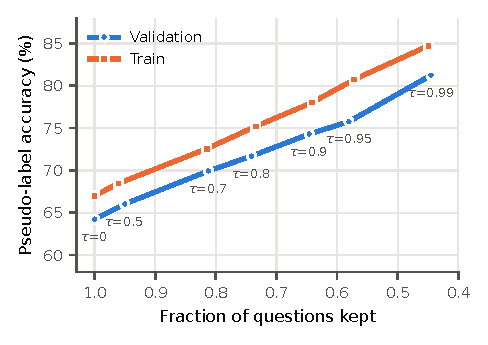
\includegraphics[width=\columnwidth]{figures/fig_tau.pdf}
\caption{Pseudo-label accuracy of the base model against the fraction of questions kept, as the softmax-confidence threshold $\tau$ increases from 0 (right) to 0.99 (left). Accuracy is measured against ground truth as a diagnostic only.}
\label{fig:tau}
\end{figure}

\subsection{Post-Fine-Tuning Results}
\Cref{tab:finetune} and \cref{fig:finetune} summarize the fine-tuning runs.

\textbf{Against the base model.} Fine-tuning on the filtered pseudo-labels leaves test accuracy exactly unchanged at 64.8\%: 13 questions are fixed and 13 are broken. Without filtering, accuracy is 65.8\% (14 fixed, 9 broken), which is not a significant difference ($p = 0.40$). Neither form of self-training improves the model.

\textbf{Against the oracle and $\tau = 0$.} Training on the same 3,985 questions with ground-truth labels raises accuracy to 77.2\%, fixing 81 questions and breaking 19 ($p < 0.001$). The fine-tuning procedure therefore works, and the difference between the filtered and oracle runs comes entirely from the labels. Of the 3,985 filtered pseudo-labels, 876 (22.0\%) are wrong; the oracle corrects them, while the filtered run trains on them. Filtering, in turn, does not help relative to $\tau = 0$: the unfiltered run is slightly better, although the difference is within noise. The training losses explain why. On the filtered set, the average loss over the first 20 updates is only 0.0045, because the model already assigns nearly all of its probability to its own confident predictions, so there is almost nothing to learn. The unfiltered set has a higher initial loss (0.074) because it includes low-confidence questions, and the oracle set has the highest (0.40) because about a fifth of its labels disagree with the model.

\begin{table*}[t]
\centering
\small
\begin{tabular}{lrrrrrrr}
\toprule
Model & Train Qs & Test acc. & Fixed / broken & McNemar $p$ & Mean $c(x)$ & Mean $c(x)$, wrong & \# $c(x) \geq 0.99$ \\
\midrule
Base (zero-shot) & -- & 64.8\% & -- & -- & 0.872 & 0.798 & 231 \\
Filtered, $\tau = 0.9$ & 3,985 & 64.8\% & 13 / 13 & 1.00 & 0.956 & 0.925 & 372 \\
No filter, $\tau = 0$ & 6,218 & 65.8\% & 14 / 9 & 0.40 & 0.954 & 0.931 & 374 \\
Oracle (gold labels) & 3,985 & \textbf{77.2\%} & 81 / 19 & $<0.001$ & 0.838 & 0.665 & 199 \\
\bottomrule
\end{tabular}
\caption{Fine-tuning results on the 500-question test subset. Fixed and broken count questions that flip from wrong to right and from right to wrong relative to the base model. Confidence is the corrected softmax confidence $c(x)$.}
\label{tab:finetune}
\end{table*}

\begin{figure}[t]
\centering
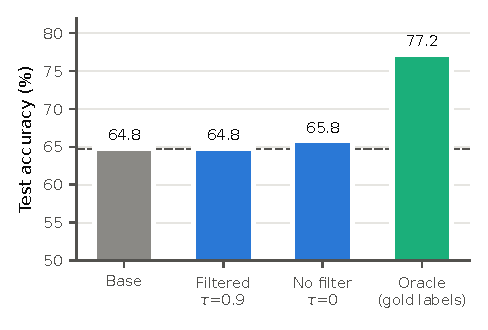
\includegraphics[width=\columnwidth]{figures/fig_finetune.pdf}
\caption{Test accuracy on the 500-question subset. The dashed line marks the base model.}
\label{fig:finetune}
\end{figure}

\subsection{Confidence Inflation and Error Propagation}
Although self-training does not change accuracy, it changes the model's confidence. After training on filtered pseudo-labels, the number of test questions with $c(x) \geq 0.99$ rises from 231 to 372, and the mean confidence on the questions the model still gets wrong rises from 0.798 to 0.925. \Cref{fig:confidence} shows this shift across the whole distribution of errors: after self-training on filtered pseudo-labels, 71\% of the remaining errors are made with confidence above 0.95, compared with 38\% for the base model. The oracle run moves in the opposite direction, lowering the confidence on its remaining errors to 0.665.

This is the mechanism behind error propagation \citep{arazo2020confirmation}. In a second round, the self-trained model would generate new pseudo-labels, and because its wrong answers are now far more confident, more of them would pass the same threshold $\tau$. Filtering by confidence would therefore become less selective with each round, even though accuracy stays flat. We plan to test this directly in the final report by measuring the pseudo-label accuracy of the self-trained model at each $\tau$, and by tracking flip rates and accuracy across rounds.

\begin{figure}[t]
\centering
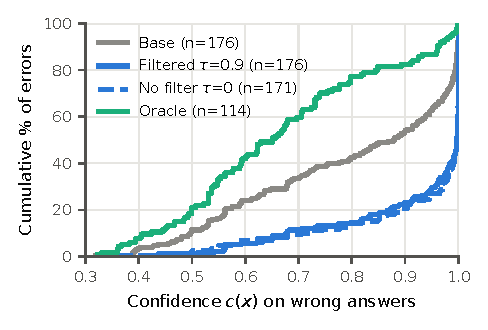
\includegraphics[width=\columnwidth]{figures/fig_confidence.pdf}
\caption{Cumulative distribution of confidence $c(x)$ on the test questions each model answers incorrectly. Curves further to the right mean more confident errors.}
\label{fig:confidence}
\end{figure}

\subsection{Comparison with Prior Work}
\citet{huang2023selfimprove} report that large language models improve by fine-tuning on their own majority-vote answers. Two differences may explain why we see no gain. First, their pseudo-labels include full chain-of-thought rationales, so training on them can teach new reasoning patterns, whereas our targets are single option letters that carry no information beyond what the model already predicts. Second, their models are orders of magnitude larger and better calibrated \citep{kadavath2022know}, while our 500M-parameter model is wrong on about 20\% of the questions it is most confident about. Our results are consistent with the confirmation-bias view of pseudo-labeling \citep{arazo2020confirmation}: without an outside signal to correct the confidently wrong labels, self-training reinforces the model's existing beliefs.

\section{Limitations and Threats to Validity}
\begin{itemize}[itemsep=1pt,topsep=2pt]
  \item \textbf{Scope.} We study a single small model, a single dataset, and one round of fine-tuning with one set of hyperparameters and one seed. The conclusions may differ for larger or better-calibrated models.
  \item \textbf{Evaluation size.} All test results use a 500-question subset, so differences of one or two points are within noise. We report paired significance tests for this reason, and will evaluate on the full test split for the final report.
  \item \textbf{Consistency signal.} All experiments use the single-pass softmax confidence. The sampled-mode signal ($k = 8$) has not been run, so we cannot yet say whether it would select different or better pseudo-labels.
  \item \textbf{Input choices.} The prompts omit the \texttt{hint} field, and image splitting is disabled. Splitting did not change base accuracy on the test subset, but it may interact with fine-tuning.
  \item \textbf{Letter bias and imbalance.} The base model predicts ``B'' on 264 of 500 test questions, while only 186 answers are ``B'' \citep{zheng2024selectionbias}. Filtering by confidence may also over-represent easier question types, which can bias the fine-tuned model.
  \item \textbf{Calibration.} The softmax confidence is informative but not calibrated (questions with $c(x) \geq 0.99$ are 81.2\% correct on validation), and we use it without recalibration.
\end{itemize}

\section{Conclusion}
We asked whether a small vision-language model can improve on visual question answering by training on its own high-consensus outputs. Reading option probabilities at the correct position gives a cheap, single-pass consistency signal that clearly separates more reliable from less reliable pseudo-labels. Fine-tuning on these pseudo-labels, however, does not improve accuracy, with or without filtering, while fine-tuning on ground-truth labels for the same questions improves it by 12.4 points. Self-training mainly makes the model more confident in what it already believes, including its mistakes, which is how errors propagate across rounds.

For the final report, we plan to (1) evaluate on the full test split, (2) compare the softmax confidence with the sampled-mode signal at $k = 8$, (3) run a second round of self-training to measure error propagation directly, (4) ablate $\tau$, the LoRA rank, and the number of epochs, and (5) test whether adding the \texttt{hint} field or recalibrating the confidence changes the outcome.

\bibliography{references}
\bibliographystyle{icml2026}

\end{document}
